\documentclass[../main.tex]{subfiles}
\begin{document}
\subparagraph{Problem 1}\label{subpar:problem1_fom}

We solve \eqref{eq:heat_fom} forward in time for $\mu\in P$ and only store the steady-state solution $\boldsymbol{u}_{h}(t=T)$ in the time-asymptotic regime $T=1$.
The various steady-states, forming the snapshots of $\boldsymbol{X}$, are depicted in Figure \ref{fig:problem1_fom}

\begin{figure}[H]
    \centering 
    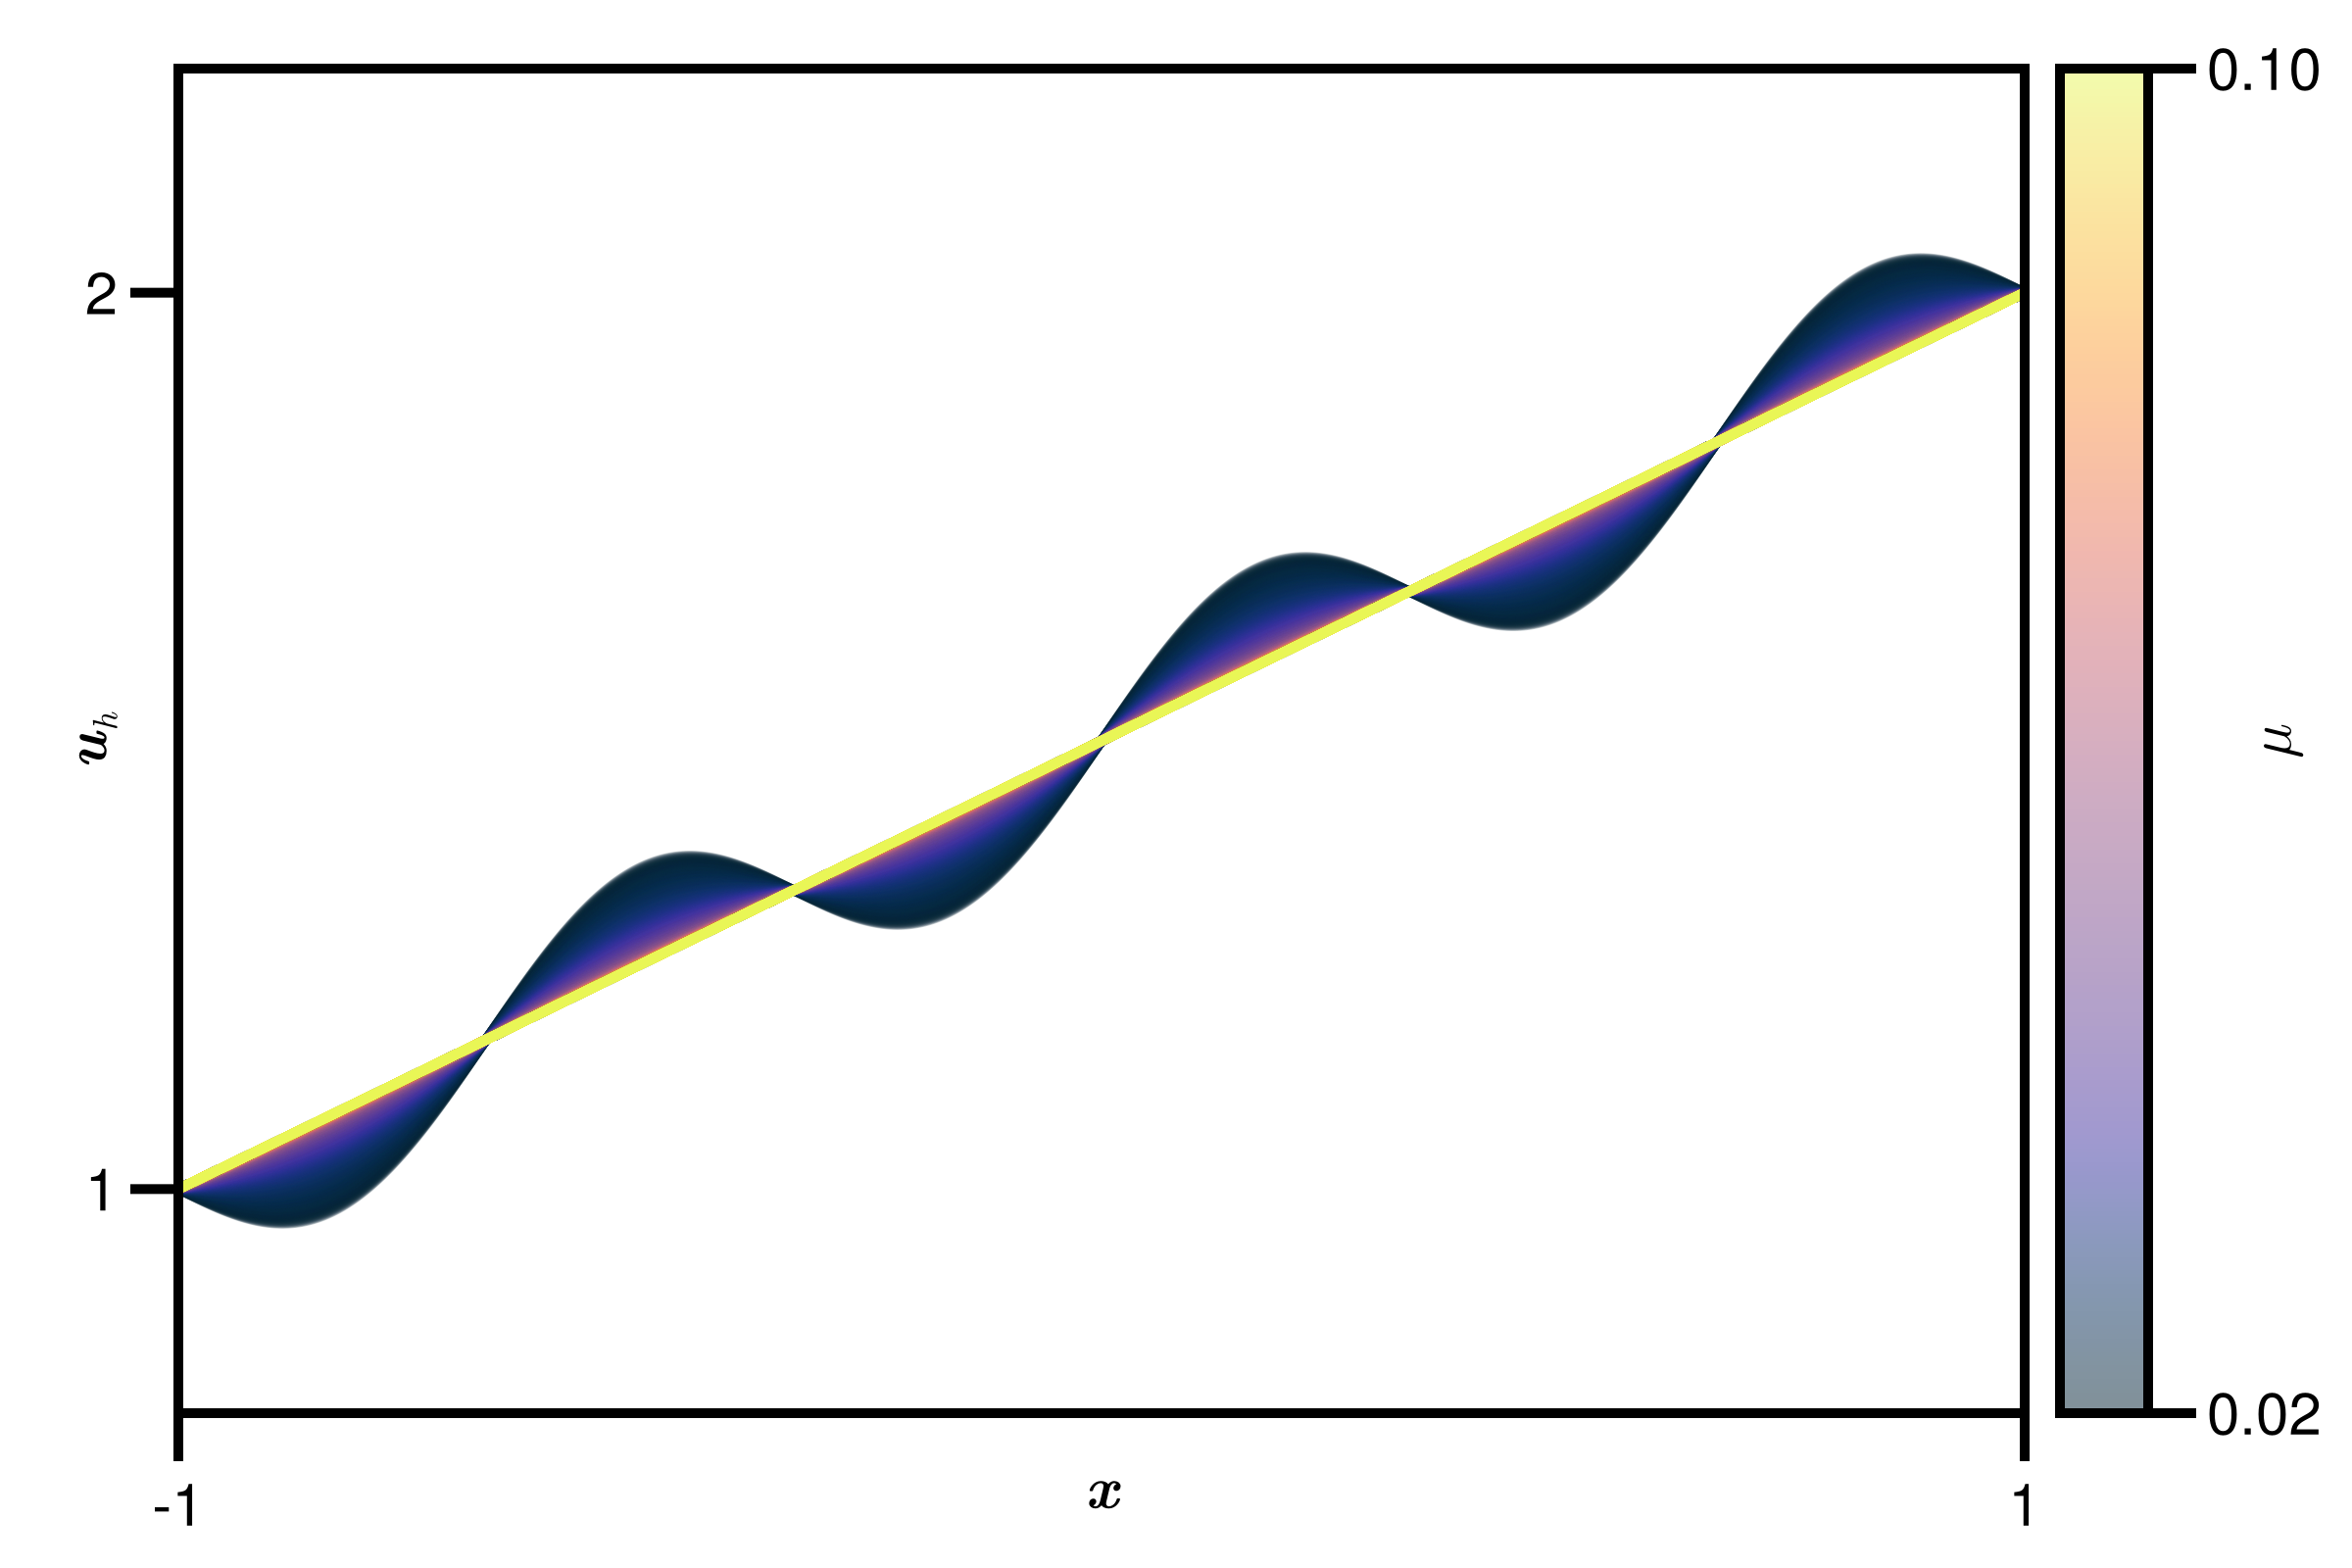
\includegraphics[keepaspectratio, width=0.7\textwidth]{../figures/fig:problem1_fom.png}
    \caption{Steady-state solutions of the FOM \eqref{eq:heat_fom} at different diffusion values.}
    \label{fig:problem1_fom}
\end{figure}

\end{document}
